
%(BEGIN_QUESTION)
% Copyright 2006, Tony R. Kuphaldt, released under the Creative Commons Attribution License (v 1.0)
% This means you may do almost anything with this work of mine, so long as you give me proper credit

Almost one century prior to Daniel Bernoulli's famous equation (1738), an Italian named Evangelista Torricelli (1643) discovered that the velocity of a liquid stream exiting a vessel was proportional to the square root of the height of the liquid column inside the vessel:

$$\includegraphics[width=15.5cm]{i00447x01.eps}$$

$$v = \sqrt{2 g h}$$

\noindent
Where,

$v$ = Liquid stream velocity, in meters per second (m/s)

$g$ = Acceleration of gravity, in meters per second squared (m/s$^{2}$)

$h$ = Height of liquid column, in meters (m)

\vskip 10pt

An interesting aspect of Torricelli's discovery was that this velocity did not depend at all on the density of the liquid.  In other words, the velocity of a mercury stream would be the same as the velocity of a water stream so long as the two liquids' column heights were equal.

It should come as no surprise that Torricelli was a student of Galileo, the man who discovered that the velocity of a falling object did not depend upon the mass of the object (neglecting the effect of air friction).

\vskip 10pt

Use algebra to prove falling objects follow the same basic rule, namely that free-fall velocity is a function of height alone and not mass (neglecting air friction):

$$\includegraphics[width=15.5cm]{i00447x02.eps}$$

Potential energy of mass at height $h$ (before falling) = $mgh$

\vskip 10pt

Kinetic energy of mass just before it hits the ground = ${1 \over 2}mv^2$

\vskip 10pt

Do you notice a similarity between the Torricelli's formula and the one you derived from the potential and kinetic energy equations?

\underbar{file i00447}
%(END_QUESTION)





%(BEGIN_ANSWER)

There is more than just a similarity here -- the two equations are absolutely identical!  This means the velocity of the liquid stream is equal to the final velocity of a falling object, if the liquid column height is the same as the object's drop height.

\vskip 10pt

Follow-up question: are the units of measurement specified for Torricelli's Theorem specific to this form of the equation, or can we use different units of measurement with the exact same equation?

%(END_ANSWER)





%(BEGIN_NOTES)

Following the principle of Energy Conservation (and neglecting air friction):

$$mgh = {1 \over 2}mv^2$$

$$gh = {1 \over 2}v^2$$

$$2gh = v^2$$

$$\sqrt{2gh} = v$$

\vskip 10pt

The units of measurement are non-specific.  Note this example in English units:

$$v = \sqrt{2 g h}$$

\noindent
Where,

$v$ = Liquid stream velocity, in feet per second (ft/s)

$g$ = Acceleration of gravity, in feet per second squared (ft/s$^{2}$)

$h$ = Height of liquid column, in feet (ft)

\vskip 10pt

Dimensional analysis confirms this:

$$\left[ \hbox{ft} \over \hbox{s} \right] = \sqrt{\left[ \hbox{ft} \over \hbox{s}^2 \right] \left[ \hbox{ft} \right]}$$

%INDEX% Physics, dynamic fluids: Torricelli's theorem

%(END_NOTES)


